%%%%%%%%%%%%%%%%%%%%%%%%%%%%%%%%%%%%%%%%%%%%%%%%%%%%%%%%%%%%%%%%%%%%
%% I, the copyright holder of this work, release this work into the
%% public domain. This applies worldwide. In some countries this may
%% not be legally possible; if so: I grant anyone the right to use
%% this work for any purpose, without any conditions, unless such
%% conditions are required by law.
%%%%%%%%%%%%%%%%%%%%%%%%%%%%%%%%%%%%%%%%%%%%%%%%%%%%%%%%%%%%%%%%%%%%

\documentclass[
  color, %% This option enables colorful typesetting. Replace with
         %% `monochrome`, if you are going to print the thesis on
         %% a monochromatic printer.
  table, %% Causes the coloring of tables. Replace with `notable`
         %% to restore plain tables.
  lof,   %% Prints the List of Figures. Replace with `nolof` to
         %% hide the List of Figures.
  lot,   %% Prints the List of Tables. Replace with `nolot` to
         %% hide the List of Tables.
  %% More options are listed in the class documentation at
  %% <http://mirrors.ctan.org/macros/latex/contrib/fithesis/fithesis/guide/mu/fi.pdf>.
]{fithesis3}
%% The following section sets up the locales used in the thesis.
\usepackage[resetfonts]{cmap} %% We need to load the T2A font encoding
\usepackage[T1,T2A]{fontenc}  %% to use the Cyrillic fonts with Russian texts.

\usepackage[
  main=english, %% By using `czech` or `slovak` as the main locale
                %% instead of `english`, you can typeset the thesis
                %% in either Czech or Slovak, respectively.
  german, russian, czech, slovak %% The additional keys allow
]{babel}        %% foreign texts to be typeset as follows:
%%
%%   \begin{otherlanguage}{german}  ... \end{otherlanguage}
%%   \begin{otherlanguage}{russian} ... \end{otherlanguage}
%%   \begin{otherlanguage}{czech}   ... \end{otherlanguage}
%%   \begin{otherlanguage}{slovak}  ... \end{otherlanguage}
%%
%% For non-Latin scripts, it may be necessary to load additional
%% fonts:
\usepackage{paratype}
\def\textrussian#1{{\usefont{T2A}{PTSerif-TLF}{m}{rm}#1}}
\usepackage{xcolor} 
\newcommand{\todo}[1]{\textcolor{red}{\textbf{#1}}}
\usepackage{listings}
\usepackage[binary-units=true]{siunitx}
%%
%% The following section sets up the metadata of the thesis.
\thesissetup{
    university    = mu,
    faculty       = fi,
    type          = bc,
    author        = Samuel Petrovič,
    gender        = m,
    advisor       = Adam Rambousek,
    title         = {The effects of age on file system performance},
    TeXtitle      = {The effects of age on file system performance},
    keywords      = {filesystem, xfs, IO operation, aging, fragmentation ...},
    TeXkeywords   = {filesystem, xfs, IO operation, aging, fragmentation ...},
}
\thesislong{abstract}{
    This is the abstract of my thesis, which can

    span multiple paragraphs.
}
\thesislong{thanks}{
    This is the acknowledgement for my thesis, which can

    span multiple paragraphs.
}
%% The following section sets up the bibliography.

\usepackage{csquotes}
\usepackage[              %% When typesetting the bibliography, the
  backend=bibtex,          %% `numeric` style will be used for the
  style=numeric,          %% entries and the `numeric-comp` style
  citestyle=numeric-comp, %% for the references to the entries. The
  sorting=none,           %% entries will be sorted in cite order.
  sortlocale=auto         %% For more unformation about the available
]{biblatex}               %% `style`s and `citestyles`, see:
%% <http://mirrors.ctan.org/macros/latex/contrib/biblatex/doc/biblatex.pdf>.
\addbibresource{citations2.bib} %% The bibliograpic database within

                          %% the file `example.bib` will be used.
\usepackage{makeidx}      %% The `makeidx` package contains
\makeindex                %% helper commands for index typesetting.
%% These additional packages are used within the document:
\usepackage{paralist}
\usepackage{amsmath}
\usepackage{amsthm}
\usepackage{amsfonts}
\usepackage{url}
\usepackage{menukeys}
\usepackage{mwe}
\renewcommand{\lstlistingname}{Example}
\renewcommand{\lstlistlistingname}{List of \lstlistingname s}


\begin{document}
\chapter{Introduction}
File systems remain an important part of modern storage solutions.  Large, growing databases, multi-media and other storage based applications need to be supported by high-performing infrastructure layer of storing and retrieving information. Such infrastructure have to be provided by operating systems (OS) in form of file system.

Originally, file system was a simple tool developed to handle communication between OS and physical device, but today, it is a very complex piece of software with large set of tools and features to go~with.

Performance testing is an integral part of development cycle of most of produced software. Because of growing complexity of file systems, performance testing took of as an important part of file system evaluation.

The standard workflow of performance testing is called out-of-box testing. Its principle is to run benchmark (e.g. testing tool) on a clean instance of OS and on a clean instance of tested file system~\cite{Traeger:2008:NYS:1367829.1367831}. Generally, this workflow present stable and meaningful results, yet, it only gives overall idea of file system behavior in early stage of its life cycle. 

File systems, as well as other complex software is subjected to progressive degradation, referred to as software aging~\cite{Cotroneo:2014:SSA:2543749.2539117}. Causes of file system aging are many, but mostly fragmentation of free space, unclustered blocks of data and unreleased memory. This degradation cause problems in performance and functionality over time. Understanding of performance changes of aged file system can help developers to implement various preventions of aging related problems.

Testing of file system aging fundamentally consists of two steps. First is to bring fresh file system to an aged state and second is the actual performance test of the aged instance.

To achieve consistency of results and to shorten testing time, file system images are used in this thesis. Once the image of an aged file system is created, it can be stored for later use. By reloading the file system image on the device, it is possible to bring the file system to the original aged state, increasing stability of results. To save space, only metadata of created file system is used, since content of created files is random and therefore irrelevant. Replayed metadata point at various blocks on device, recreating fragmentation while seldom taking significantly less space.

Foremost, this thesis describe implementation of flexible tests which represent the two aforementioned steps. The first test is able to age fresh file system and store the result as an image for later use. The performance statistics collected in the process, as well as resulting layout can be used to evaluate ability of file system to respond to aging. Second test can evaluate resulting image even further by releasing some space and conducting performance test on resulting layout. 

Furthermore, using developed tests to test different configurations of file systems and storage is demonstrated. The subject of research are differences between popular Linux file systems (XFS, Ext4) and storage technology (HDD, SSD) in context of aging. Because of nature of collected data, a processing tool was implemented to parse large amount of information into human readable reports. All the generated reports are part of this thesis in form of Appendix A.

The aging tests implemented in this thesis are established as part of testing cycle in Red Hat Kernel Performance team.

In the second chapter, the text present already conducted research of effects of age and fragmentation on file system performance. Third chapter describes used file systems and theirs main features. Chapter 4 introduce tools used in implementation of tests while describing their relevant features. Chapters 5 and 6 describe actual implementation of mentioned tests and remaining chapters present the results obtained by using created tests. In the conclusion chapter, I discuss the effects of age on file system performance as well as further options for file system aging performance testing.

\chapter{Related work}
In this chapter I present different approaches of file system aging and fragmentation research described and implemented in the past. The first section discuss usage of collected data to create aging workload. The second section discuss possibilities of aging the file system artificially, without pre-collected data.

\section{Aging file system using real-life data}
This approach is based on modeling the aged file system using data collected from file systems used in real-life environment.

Such data can be in form of snapshots (e.g. images) of file systems, as was thoroughly described by Smith and Seltzer~\cite{Smith:1997:FSA:258623.258689}.

The snapshots were collected nightly over a long period of time (one to three years) on more then fifty file systems. By comparing pairs of snapshots in the sequence, performed operations were estimated, resulting in a very realistic aging workload. However, as some studies suggest, most of files have life span shorter than 24 hours~\cite{Ousterhout:1985:TAU:323647.323631}. Therefore, as Smith and Seltzer admit, by snapshoting every night, this process does not account for most of the created files, resulting in loss of important part of data.

Furthermore, to age a file system sized $\SI{1024}{\mega\byte}$, $\SI{87.3}{\giga\byte}$ of data had to be written, taking 39 hours to complete, rendering the workflow impractical for in-production testing needs.

Smith and Seltzer also defined a layout score as a method to evaluate fragmentation of a file system. Layout score is defined as a fraction of blocks of file, which are contiguously allocated. Files of one block size are ignored, since they can't be fragmented, and for every file, first block is ignored too. Evaluation of the whole file system is then computed as an aggregated layout score of all files.

The problem resulting from not tracking shortly lived files can be solved by another approach called collecting traces. Traces are sequences of I/O operations performed by OS, captured at various levels (system call, drivers, network, etc.). The sequence of operations can be replayed back to the file system, aging it in a realistic manner.

Overall, using real-life data to age file systems brings realistic results, but at a cost of higher expenses, such as storing the collected data (metadata snapshot of $\SI{500}{\giga\byte}$ Ext4 file system can have up to $\SI{500}{\mega\byte}$). Additionally, to cover cases of different types of file system usage, data from several such file systems have to be collected, expanding the amount of needed data even further. Such data is not always available, rendering this type of approach useful only in cases the researcher is already in possession of said data.

\section{Synthetic aging simulation}
Synthetic aging is a type of aging that does not require real-life data for its running. It relies on purely artificial workload performed on a file system, invoking aging factors, such as fragmentation.

Fast file system aging was described as a part of a trace replay benchmark called TBBT~\cite{Zhu:2005:TSA:1251028.1251052}. This type of aging consists of sequence of interleaving append operations on a set of files. By controlling the amount of files involved in the process, researchers had great control over fragmentation. Such workflow, while creating desired fragmentation, is however quite unrealistic, making the results of testing on such file system questionable~\cite{Traeger:2008:NYS:1367829.1367831}.

The way to conduct synthetic aging, while keeping some amount of realism is to try to mimic the real-life usage by creating requests of random nature. 

Aging workload generator such as fs-drift~\cite{fs-drift:github}, used in this thesis, can be used (while carefully configured) to mimic long term real-life usage. Fs-drift simply creates a sequence of randomly chosen requests to be handled by the file system. The probability of the request type to be chosen is controlled by the workload table. In addition, whole process is highly configurable, making it possible to simulate various types of file system usage. Furthermore, a random distribution of file access can be controlled to mimic real-life user. All mentioned qualities, if used correctly, could result in fast, real-life mimicking file system aging.








%%The standard workflow is tu run benchmark clean instance of operating system without other applications running, to avoid noise, and on clean instance of researched file system.

%%While this approach brings great results, with correct configuration of the benchmark, it only gives researchers a general idea about how does file system perform in early stage of it's usage. 

%%However, there is a growing demand from users as well as from file system developers to explore behavior and performance of a file system, that has been used for longer period of time.



%%This introduces problem in regard of devices with moving parts, such as widely used hard disk drive. When working with I/O operations on this type of device, the fragmentation cause larger seek times, which is a time for magnetic heads to reach desired location. This is a great example of how file system has to be flexible to solve such problems as well as of problems that emerge after running file system for a longer period of time.

%%The ideal approach of research pointed on effect on age of file system would be to put file system under defined conditions for a few years or months, gathering information in the process. However, this is apparently impractical or even impossible, because the demand for results has to be satisfied in matter of weeks to respond to new versions of file systems, which are developed and released quite often.

%%One of the earliest ideas about how to deal with this problem would be to capture a snapshot of a file system that had already been used for a prolonged time. This approach of testing on such a snapshot, however, would probably lead to optimising for a very specific instance of old version of given file system. 

%%If researchers want to predict behavior of a new version of file system after prolonged time of usage, they should be able to create a simulation, which would mimic the aging process, but in short period of time.
%%Aim of this thesis is to create 
%%This can be technically implemented, because the idea is to run the simulation continuously under very heavy workload without using operations which does not alter file systems layout, therefore researchers should be able to compress the time of creating such an aged file system in a short period of time.

%%Unfortunately the demand from users and developers has yet not been met by standard studies. There has been few studies executed in last millenium, that shed some light on this topic, but overall, modern research is in hands of regular users, remaining in amateur sphere, lacking professional equipment to execute such research properly.

%%The aim of this thesis is to create standard, configurable workflow of creating and storing aged file system as well as a workflow to mesure its performance. Workflow for file system aging will use open source tool fs-drift to simulate aging process and then creates and stores file system image using system tools. Workflow for performance testing will then use created images to perform various tests.

%%These workflows will then be used to test XFS and EXT4 file systems on different storage media to show their strenghts and weaknesses in respect to long time runnign, while showing importance of this kind of testing.

%%The conclusion of research will show how does aging affect hard drive disks compared to solid state disks, what effect has aging on file system performance and what are the performance differences between XFS and EXT4 after long time usage.

%%The workflows created for this thesis will be included in Red Hat File system performance testing campaigns.


\chapter{File systems}
In this chapter, I present basic information about file systems and describe main features of chosen file system in regard of fragmentation and scalability, which are important topics when discussing file system aging.

File system is a set of tools, methods, logic and structure to control how to store and retreive data on and from device.

The system stores files either continuously or scattered across device. The basic accessed data unit is called a block, which capacity can be set to various sizes. Blocks are labeled as either free or used.

Files which are non-contigous are stored in form of extents, which is one or more blocks associated with the file, but stored elsewhere.  

Information about how many blocks does a file occupy, as well as other information like date of creation, date of last access or access permissions is known as metadata, e.g. data about stored data. This information is stored separately from the content of files. On modern file systems, metadata are stored in objects called index nodes (e.g. inodes). Each file a file system manages is associated with an inode and every inode has its number in an inode table. On top of that the file system stores metadata about itself (unrelated to any specific file), such as information about bad sectors, free space or block availability in a structure called superblock.

In this thesis, targeted file systems are two most popular Linux file systems~\cite{Lu:2013:SLF:2591272.2591276}, XFS~\cite{xfs:qhe} and Ext4~\cite{ext4:qhe}, which are also main Red Hat supported file systems. These file systems belong to the group of file systems called journaling file systems.

Journaling file system keeps a structure called journal, which is a buffer of changes not yet commited to the file system. After system failure, these planned changes can be easily read from the journal, thus making the file system easily fully operational, and in correct and consistent state again.

\section{XFS}
XFS is a 64-bit journaling file system known for its high scalability (up to 9 exabytes) and great performance. Such performance is reached by architecture based on allocation groups.

Allocation groups are euqally sized linear regions within file system. Each allocation group manages its own inodes and free space, therefore increasing parallelism. Architecture of this design enables for significant scalability of bandwidth, threading, and size of file system, as well as files, simply because multiple processes and threads can access the file system simultaneously.

XFS allocates space as extents stored in pairs of B+ trees, each pair for each allocation group (improving performance especially when handling large files). One of the B+ trees is indexed by the length of the free extents, while the other is indexed by the starting block of the free extents. This dual indexing scheme allows efficient location of free extents for I/O operations.

Prevention of file system fragmentation consist mainly of a features called delayed allocation and online defragmentation.

Delayed allocation, also called allocate-on-flush is a feature that, when a file is written to the buffer cache, substracts space from the free-space counter, but won't allocate the free-space bitmap. The data is held in memory until it have to be stored because of system call. This approach improves the chance, that the file will be written in a contiguous group of blocks, avoiding fragmentation and reducing CPU usage as well.

\section{Ext4}
Ext4, also called fourth extended filesystem is a 48-bit journaling file system developed as successor of Ext3 for Linux kernel, improving reliability and performance features. Ext4 is scalable up to 1 exbibyte (approx. 1.15 exabyte). Traditional Ext2 and Ext3 block mapping scheme was replaced by extent based approach similar to XFS, which positively affects performance.

Similarly to XFS, Ext4 use delayed allocation to increase performance and reduce fragmentation. For cases of fragmentation that still occur, Ext4 provide support for online defragmentation~\cite{sato2007:ext4} and e4defrag tool to defragment either single file, or whole file system.

\chapter{Used tools}
In this chapter, I presnet tools which were used to implement automated tests for creating and storing aged file systems and measuring their performance. Furthermore, I describe the main features and means of their usage. All the presented tools are open source projects.

\section{Beaker}
Beaker is an open source project aimed at automating testing workflow. The software can provision system from a pool of labs, install OS and packages, configure environment and perform tasks. The whole process is guided by sequence of instructions in an XML format. Examples can be found in Apendix A.





\section{FIO}
Flexible Input/Output tool is a IO workload generator written by Jens Axboe. It is a tool well known for it's flexibility as well as large group of users and contributors. The flexibility is integral for conductuing less artifical and more natural performance tests. However, approaching more natural test behavior, stability of results drop, so ideal equilibrium between these two requirement has to be found.

FIO accept the workload specification as either a configuration file or a single line. Multiple different jobs can be specified as well as global options for every job. 

The benchmark creates requests on system level, allowing for great power over the generated workflow.

There is a possibility to choose from 4 I/O operations to be performed (or their mix). These operations are sequential write, sequential read, random write and random read. Verification of the issued data is offered as well. Size of generated file and block size can be controlled too and it can be either stable or chosen from given range. For cache-tiering workloads, different random distributions (f.e. Zipf) can be specified. FIO also supports process forking and threading.

After the test, FIO will compute overall report of measured performance. However, logging of multiple properties can be enabled, giving researchers even more oversight about the nature of file system performance.

\section{Fs-drift}
Fs-drift is a very flexible aging test, which can be used to simulate lots of different workloads. The test is based on random file access and randomly generated mix of requests. These requests can be writes, reads, creates, appends, truncates or deletes.

At the beginning of run time, the top directory is empty, therefore \textit{create} requests success the most, other requests, such as \textit{read} or \textit{delete}, will fail because not many files has yet been created. Over time, as the file system grows, \textit{create} requests began to fail and other requests will more likely succeede. File system will eventually reach a state of equilibrium, when requests are equaly likely to execute. From this point, the file system would not grow anymore, and the test runs unless one of the stop conditions are met.

The mix of operation probabilities can be specified in separate csv file. Fs-drift will try to issue more \textit{create} operations at the beggining of testing, so other operations execute with higher likeliness.

The file to perform a request on is randomly chosen from the list of indexes. If the type of random distribution is set to \textit{uniform}, all indexes have the same probability to be chosen, see \ref{fig:rand1}. However, if the type of random distribution is set to \textit{gaussian}, the probability will behave according to normal distribution with the center at index 0 and width controled by parameter \textit{gaussian-stddev}. This is usefull for performing cache-tiering tests. Please note, that file index is computed as modulo maximal number of files, therefore instead of accessing negative index values, the test access indexes from the other side of spectrum, see Figure \ref{fig:rand2}

Furthermore, fs-drift offers one more option to influence random distribution. After setting parameter \textit{mean-velocity}, fs-drift will choose files by means of moving random distribution. The principle relies on a simulated time, which runs inside the test. For every tick of the simulated time, the center of bell curve will move on the file index array by the value specified using \textit{mean-velocity} parameter. By enabling this feature, the process of testing moves closer to reality by simulating more natural patterns of file system access (the user won't access file system randomly, but rather works with some set of data at a time). On Figure \ref{fig:rand3}, you can see bell curve moving by 5 units two times.

\begin{figure}[!htb]
    \centering
    \begin{minipage}{\textwidth}
        \centering
        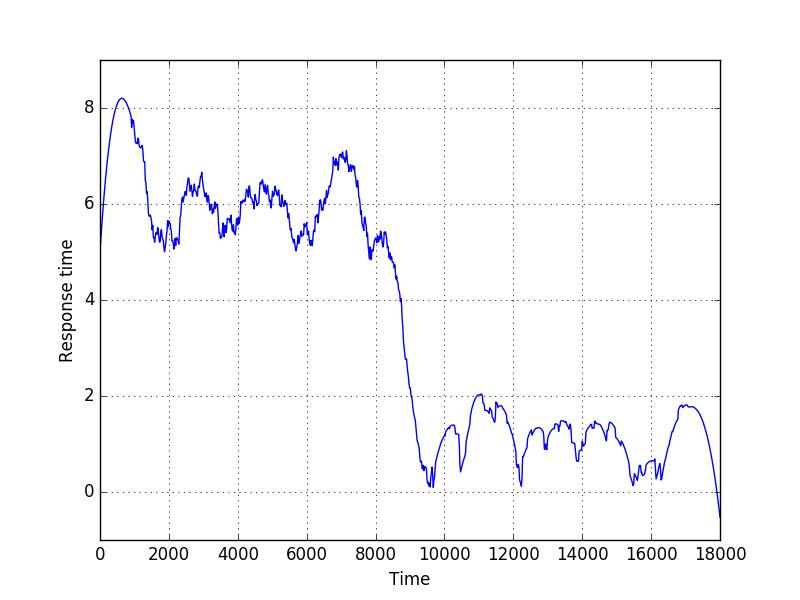
\includegraphics[width=0.7\textwidth]{../scripts/fig1.png}
        \caption{Uniform distribution of file access}
\label{fig:rand1}
    \end{minipage}\hfill
    \begin{minipage}{\textwidth}
        \centering
        \includegraphics[width=0.7\textwidth]{../scripts/fig2.png}
        \caption{Normal distribution of file access}

\label{fig:rand2}
    \end{minipage}

\end{figure}
\begin{figure}
    \begin{minipage}{\textwidth}
        \centering
        \includegraphics[width=0.7\textwidth]{../scripts/fig3.png}
        \caption{Moving random distribution}
\label{fig:rand3}
    \end{minipage}
\end{figure}

For purpose of this thesis, several changes had to be made to the original code. Besides small errors like invalid Readme information, a bug in code had to be repaired, otherwise the fs-drift would not delete files while issuing \textit{delete} operation, marginally affecting aging process. Without this fix, the volume would just saturate and remain in more or less consistent state for the rest of the runtime.

Additionally, to be able to inspect and work with the file system while aging process is still running, I added an option to specify \textit{pause file}. If the pause file is present, the fs-drift would not issue any requests and waits until the file is removed\footnotemark[1].
\footnotetext[1]{For all the changes made to master branch of fs-drift, see ...}

Fs-drift offers even more parameters to control the test run such as number of directories, levels of directories, or enabling \textit{fsync}/\textit{fdatasync} to be called. To stop the fs-drift, one of the stop conditions have to be met. The stop condition can be either reached maximal number of performed operations, running out of time, or apparance of stop file.

For evaulation of the aging process, fs-drift can log latency of the performed opperations. However, the log doesn't differentiate between the operations, which could be usefull for further research.

Used configuration of fs-drift for purposes of aging testing is further described in chapter 4.

\subsection{Changes to original code}
Several changes had to be made to the original code prior to testing.

The most obvious problem with the tools was, that it did not conduct \textit{delete} operations. As stated, deleting files is quite crucial to file system aging.

Another problem emerged when gathering statistics of response time evolution through the aging process. Since the tool is generating the I/O requests at random, sometimes, error occurs. Most operations (except \textit{create}) need the file to exist to success, but sometimes, the file is non-existent. The problem with response time logging was, it logged the response time even if the operation didn't carry, causing noise to the data.

Further problem with response time logging was, it didn't differentiate between operations. Such distinction could greatly affect the way researchers can find problems with file system evolution.

As mentioned, possibility of specifying \textit{pause file} was added, making the fs-drift easy to pause for file system contents inspection.

Another feature added to fs-drift was non-uniform distribution of file sizes. Originally, fs-drift just used \textit{randint} to uniformly choose file size at interval 1 to \textit{maximum\_file\_size}. Such implementation offers very little control over file size distribution. Therefore, possibility to specify array of weights was added, so fs-drift can choose file size at different distribution.

The version used for testing in this thesis have all the mentioned problems repaired and features implemented.

\section{Storage generator}
Storage generator is a beaker task developed by Jozef Mikovič. It is capable of automated configuration of storage on a machine. In a single-device mode, storage generator simply creates new partition on a given device and creates and mounts file system. In a recipe mode, storage generator follows set of bash instruction to create more advanced configurations such as merging multiple devices using LVM, creating LVM cache or encrypted volume.

The creation of XFS file system is standard, but Ext4 file system is created with additional option, disabling \textit{lazy init}. \textit{Lazy init} is a feature which allows for fast creation of file system by not allocating all the available space at once. The space is allocated later, as the file system grows. Such additional allocation, however would skew data collected in the first hours of the test, therefore it is disabled in these tests.



\chapter{Creating aged file system}
In this chapter, I describe process of developement of file system aging workflow and its implementation as a form of automated test.

\section{Aging process}
As mentioned, fs-drift was used as a mean of aging the fresh file system, bringing it to the aged, fragmented state. Fs-drift is quite flexible, therefore a lot of parameters and their impact on the final block layout had to be considered.

First, the amount of fullness had to be taken into account. Heavily used file systems tend to be full at amounts ranging from 75 to 100 percent~\cite{agrawal2007five}. However, fs-drift does not offer an option to directly control the fullness of the file system. As the creator states in README, to fill a file system, maximum number of files and mean size of file should be defined such that the product is greater than the available space. Parameters to overload the volume are not difficult to come up with. The problem is, the random nature of the test doesn't allow for meaningfull reporoducibility of the reached equilibrium. In most cases, fs-drift plainly saturates given volume, so used space remains at 100\% through the rest of the testing time. This drawback was overridden by a small change in fs-drift code\footnotemark[1]. By adding the possibility to specify a \textit{pause file}, other processes can stop fs-drift to generate IO requests for some time. This allows asynchronous thread triggered before fs-drift to pause it, when the file system usage reaches a specified amount and free some space.

\footnotetext[1]{For all the changes made to master branch of fs-drift, see Chapter 3}

In fs-drift, there is an option to define a workload table, describing probability of used operations. Since the goal of this workload is to create fragmented file system in a short time, operations which do not alter file system block layout are not included. Only create, delete, append, trucate and random write have representation in this workload. 

File size is another important factor of succesfull simulation. To consider the simulation succesfull, resulting layout should have similar file size distribution as real-life file systems. File size is distributed non-uniformly in real-life file systems, so to achieve realistic file system layout, file size distribution has to be non-uniform during the test.

As a reference for file size distribution, five year old study of file system metadata was used~\cite{agrawal2007five}. Figure 3 shows measured file size distribution of used file systems. To mimic this layout, I modeled bimodal random distribution with modes at $\SI{8}{\mebi\byte}$ and $\SI{1}{\gibi\byte}$. The shape of resulting distribution in shown in figure~\ref{fig:bimodal}.

\begin{figure}[!htb]
    \begin{minipage}{\textwidth}
        \centering
        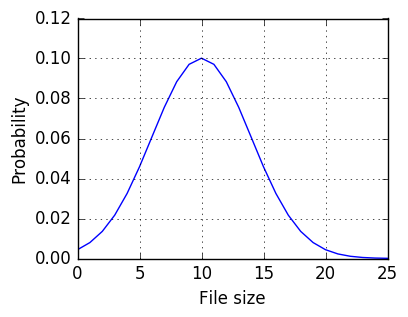
\includegraphics[width=0.7\textwidth]{../scripts/dist.png}
        \caption{Bimodal distribution of file size}
\label{fig:bimodal}
    \end{minipage}
\end{figure}

%The optimal results were reached when every operation had equal representation, e.g. 33\%

%The fs-drift allows directories up to defined level to create.

%The directory in which a file is directly affect its chance to be selected for a chosen operation, so by using only one directory, the equilibrium happens too fast, long before the file system is filled completely. Therefore we allow up to three levels of directories to be created.

Duration of the test is set to 5 hours for the pilot testing and 10 hours 

\section{File system images}
File system images can be created by using tools developed to inspect file systems in case of emergency. For Ext* file systems, there is a tool called \textit{e2image} and for XFS, \textit{xfs\_metadump} and \textit{xfs\_mdrestore}. Both tools create images as sparse files, so compression is needed.

\textit{E2image tool} can save whole contents of a file system or just its metadata and offers compresion of image as well. Created images can be further compressed by tools such \textit{bzip2} or \textit{tar}. Such images can be later replayed back on a device. From that point, file system can be mounted and revised.

\lstset{language=bash, 
numbers=none, 
frame=single, 
commentstyle=\color{dkgreen}, 
basicstyle={\scriptsize\ttfamily}, 
keywordstyle=\color{blue}, 
%identifierstyle=\color{blue}, 
stringstyle=\color{red},
captionpos=t,
showstringspaces=false,
breaklines=true,
breakatwhitespace=false,
tabsize=3,
caption={sdad},
}

\begin{lstlisting}[language=bash, caption={Creating compressed image using \textit{e2image}}][frame=single]
  $ e2image -Q $DEVICE $NAME.qcow2
\end{lstlisting}

\begin{lstlisting}[language=bash, caption={Reloading compressed image}][frame=single]
  $ e2image -r $NAME.qcow2 $DEVICE
\end{lstlisting}

\textit{Xfs\_metadump} saves XFS file system metadata to a file. Due to privacy reasons file names are obsfucated (this can be disabled by -o parameter). As well as \textit{e2image} tool, the image file is sparse, but \textit{xfs\_metadump} doesn't offer a way to compress the output. However, output can be redirected to stdout and compressed further on. Generated images, when uncompressed, can be replayed back on device by tool \textit{xfs\_mdrestore}. File system can be then mouned and inspected as needed.

\begin{lstlisting}[language=bash, caption={Creating compressed image using \textit{xfs\_metadump}}][frame=single]
  $ xfs_metadump -o $DEVICE -|bzip2 > $NAME
\end{lstlisting}

\begin{lstlisting}[language=bash, caption={Reloading image using \textit{xfs\_mdrestore}}][frame=single]
  $ xfs_mdrestore $NAME $DEVICE
\end{lstlisting}

%\section{filesystem\_ager}
%This aging tool is a simple approach to write and remove many files of random size.

%The tool consist of three scripts and one common library called \textit{functions}. The scripts are named \textit{filesystem\_ager.py}, \textit{fio\_config\_generator.py} and \textit{random\_deletor.py}.

%The workflow consist of calling filesystem\_ager, with desired parameters. Script manages triggering fio\_config\_generator, calling fio tool on generated config and triggering random deletor. These three actions are repeated given number of times.
%Parameters of filesystem\_ager are: 
%\begin{compactenum}
%  \item Total desired size do be written in one cycle
%  \item Denominator of total desired size (Total desired size will be divided by this number)
%  \item Range of size of written files
%  \item Number of cycles
%\end{compactenum}

%Although FIO tool has some parameters to randomize the size of files which are written, the management of file sizes and randomisation, as well as naming of files is handled by fio\_config\_generator instead, to provide more control over those qualities.
%Parameters of this script are:
%\begin{compactenum}
%  \item Total deisred size to be written
%  \item Range of size of written files
%\end{compactenum}

%The script will generate global settings of a workload, then proceeds to generate jobs for every file that will be written. File size is always the name of that file, and these are gathered to a list, then list of generated files is returned and script ends. Including file size in its name, as well as indexation of files will help effectively search and delete files in the random deletion process, without need to search for files on the disk and examine them for size. Simplistic approach in fio config will hopefully result in compatibility and reliability in use with any fio version.

%After config file is generated, filesystem\_ager will run fio tool on generated config and therefore, files are written on the device.

%The removing of files is handled by random\_deletor script. Its parameters are:
%\begin{compactenum}
%  \item Total written size
%  \item Denominator of total size
%  \item Range of size of written files
%  \item Number of existent files
%\end{compactenum}

%If denominator equals zero, random\_deletor wont remove any files and will return empty list. Otherwise, desired range of deletion is estimated. Random\_deletor then proceeds to remove files while desired volume is not deleted. Files are randomly selected through choosing random integer from zero to number of existent files. This step may seem inefficient, but with large amounts of generated files, the time to perform succesfull selection will not change dramatically. Selected file name is then parsed for size information, and if it fits into desired volume to remove, it is deleted, through subprocess command. Names of removed files are gathered in a list and returned.

%Number of deleted files is substracted from number of existent files.
%filesystem\_ager then sums up deleted volume, log it as well as other information and triggers the cycle again.

%However, after few runs, I decided not to use this approach for actual aging, because the time needed to fill and appropriately age the filesystem simply took very long. Instead, I was looking for other, already created tools I could use.

\section{Implementation details}
Workflow of image creating is contained in the Beaker task drift\_job. After extracting fs-drift, the main script starts python script, which handles the process of running fs-drift. Settings of fs-drift are passed as a parameter and then parsed inside the script. Before running the fs-drift, asynchronous thread is triggered to periodically log free space fragmentation and file system usage while fs-drift is running. If the usage reaches --hranica-- specified amount of space si freed from file system\footnotemark[2].

\footnotetext[2]{The mechanism of freeing space from file sytem is described in next chapter}

After the fs-drift ends, image of file system is created using presented tools, and archived using \textit{bzip2}. All the generated data and information about environment is archived as well and text file describing the test is generated. These three files are then sent (via \textit{rsync}) to the specified destination.

Parameters available for drift\_job:
\begin{compactenum}
  \item -s, --sync, flag to signalise weather or not to send data to server (usefull for developing purposes)
  \item -M, --mountpoint
  \item -d, --disk, device usded during test
  \item -r, --recipe, parameters to pass to fs-drift
  \item -t, --tag, string to distinguish different storage configurations
  \item -q, --drifttype, string to distinguish different aging configurations
  \item -m, --maintain, parameter to specify maximum volume usage and amount to be freed
  \end{compactenum}

\chapter{Performance testing of aged file system}
In this chapter, I describe structure of performance test which use images created by previous workflow. In the first section, I present settings of FIO benchmark for the optimal results and in section two, I describe implementation of this test as beaker task.

\section{Benchmark settings}
To ensure stability of test results, simple form of standard performance test was used.
%Volume is randomly removed using random\_delete\_volume.py script. This scriptt globs all files in the filesystem, retrieves information about used volume as well as it's overall size. Then proceeds to randomly choosing files to delete and stops when desired volume is freed. The approach of recursively globbing all files may be inefficient, but this way, we can be sure, that volume is deleted from whole device evenly.

%\section{Inspecting filesystem}

%To determine overall idea about an extent to which is the file system aged, scripts that generate histograms representing fragmentation of used space as well as fragmentation of free space. Both scripts use common linux tools and pyplot to generate the graphics. Both scripts can display linear or logarhytmic Y scale.

%Script extent\_distribution.py makes use of xfs\_io fiemap tool, which is a tool to display extent distribution of a given file and works correctly even for ext* filesystems.

%The script will first recursively crawls the whole filesystem from given top folder and makes a list of all files. Fiemap is then run over every file separately. 

%The only data, that are then parsed from the output, is how many non-contigous extents does the file have. These integers are aggregated to a single list, from which are then counted, and final histogram is made.

%Script free\_space\_fragmentation.py use the tool e2freefrag, which runs over a device, and outputs the histogram of free space fragmentation in texutal form. Script will store this output and then easily parse the histogram and aggregate the data into a graphic form.

\section{Test structure}
Performance testing of created images is done by a package recipe\_fio\_aging. Upon instalation of necessary tools (libs, fio), the package finds and downloads coresponding file system image according to obtained parameters. As shown, images are stored compressed, therefore decompression is needed after download. Once these steps are succesfully completed, the image is restored on the device by using presented tools (e2image, xfs\_mdrestore). If the image restoring completes succesfully, file system can be mounted and worked with exactly like it would be just after the aging process.

After image restoration, some amount of the files needs to be deleted to create space for the performance test to take place. The files to be removed are chosen randomly until desired amount of volume has been freed. By using this workflow, e.g. freeing some amount of space, we can simulate aged file system in various phases of aging by using just one image of a very fragmented file system.

When free space is reclaimed, FIO test will take place using parameters given to recipe\_fio\_aging. The overall space occupied by the test should not be larger than available space on the file system, otherwise the test will either fail completely or report incorrect results.

For statistical correctness, the FIO test can run several times in a row. After last iteration, the results are archived and sent to data-collecting server.

Parameters available for recipe\_fio\_aging:
\begin{compactenum}
  \item -s, --sync, flag to signalise wheather or not to send data to server (usefull for developing purposes)
  \item -n, --numjobs, number of test repetitions. For statistical stability
  \item -m, --mountpoint
  \item -d, --device
  \item -r, --recipe, parameters to pass to FIO test
  \item -t, --tag, string to distinguish different tests
  \end{compactenum}

\chapter{Testing environment}
In this chapter, I describe testing environment and storage used for testing with created tests.

\begin{tabular}{|l|l|}
\hline
   \multicolumn{2}{|l|}{Machine1} \\ \hline
    Model & Lenovo\texttrademark System x3250\,M6 \\
    \hline
    Processor & Intel\textsuperscript\textregistered Xeon\textsuperscript\textregistered E3-1230\,v5 \\
    \hline
    Clock speed & $\SI{3.40}{\giga\hertz}$ (4 cores) \\
    \hline
    Memory & $\SI{1628}{\mega\byte}$ \\
    \hline
    \multicolumn{2}{|l|}{Storage} \\ \hline
    Device & HP Proliant HardDrive EG0600FBVFP \\ \hline
    Interface & SAS\\ \hline
    Capacity & $\SI{600}{\giga\byte}$\\ \hline
\hline
   \multicolumn{2}{|l|}{Machine2} \\ \hline
    Model & Lenovo\texttrademark System x3250\,M6 \\
    \hline
    Processor & Intel\textsuperscript\textregistered Xeon\textsuperscript\textregistered E3-1230\,v5 \\
    \hline
    Clock speed & $\SI{3.40}{\giga\hertz}$ (4 cores) \\
    \hline
    Memory & $\SI{1628}{\mega\byte}$ \\
    \hline
    \multicolumn{2}{|l|}{Storage} \\ \hline
    Device\,1 & HP Proliant HardDrive EG0600FBVFP \\ \hline
    Interface & SAS\\ \hline
    Capacity & $\SI{600}{\giga\byte}$\\ \hline
    Device\,2 & SSD \\ \hline
    Interface & SATA\\ \hline
    Capacity & $\SI{120}{\giga\byte}$\\ \hline
\hline
   \multicolumn{2}{|l|}{Machine3} \\ \hline
    Model & IBM x3650 System\,M4 \\
    \hline
    Processor & Intel\textsuperscript\textregistered Xeon\textsuperscript\textregistered E5-2620\,v2 \\
    \hline
    Clock speed & $\SI{2.10}{\giga\hertz}$  (4 cores) \\
    \hline
    Memory &  $\SI{65536}{\mega\byte}$\\
    \hline
    \multicolumn{2}{|l|}{Storage} \\ \hline
    Device\,1\&2 & IBM Solid State Drive SSDSC2BB480G4i\\ \hline
    Interface &  SATA\\ \hline
    Capacity & $\SI{400}{\giga\byte}$\\ \hline

\end{tabular}

Installation of system and configuring is done using tools presented in Chapter 3. 

The system installed on machines is RHEL-7.3 with kernel 3.10.0-514.el7.x86\_64

\section{Storage}

\subsection{Hard disk drive}
A hard-disk drive is a type of storage device which use one or more magnetic plates to store and retreive data. Desired physical address can be reached by rotating the plates and positioning magnetic read-write heads. The plates rotate at stable speed at around 7500rpm (even more for enterprise-level hardware).

Since the parts of HDD have to physically move to reach desired address, there is a latency to the data access. The time for magnetic head to find next relevant block of data is called a \textit{seek time}. Because the length of seek time has significant impact on overall I/O performance, OS have to do a lot of optimising, such as pre-fetching.

Obviously, block layout would have a large impact on performence of this kind of device. The amount of fragmentation (thus aging) affect the number of performed seeks. This cause the pressure on file system to store data more contiguously and also cluster related data.

\subsection{Solid state drive}
As for SSD, this type of device does not have any moving parts, which make perform really well. One of the problems, however, is limited lifecycle of memory cells. SSD manufacturers deal with this problem by adding controler with its own scheduler, which make sure, no parts of the device are used significantly more than other parts.

%When aging the filesystems, I expect for those grown on HDD to perform significantly slower after aging process, and I expect SSD filesystems not to be affected at all, or maybe significantly less.

\chapter{Results}

\section{Performance of aged file system}
\section{Differences betweem XFS and EXT4}
\section{Differences accross different storage}
\chapter{Conclusion}
Here I will admit, that these results were not really surprising and ABSOLUTELY no breakthrough, however, as noone really research this branch of QE, the results are definitely a step further in this field.

\printbibliography

\appendix %% Start the appendices.
\chapter{Reports}
\chapter{Examples}
\lstset{language=XML, 
numbers=left, 
frame=single, 
commentstyle=\color{dkgreen}, 
basicstyle={\scriptsize\ttfamily}, 
keywordstyle=\color{blue}, 
%identifierstyle=\color{blue}, 
stringstyle=\color{red},
captionpos=t,
showstringspaces=false,
breaklines=true,
breakatwhitespace=false,
tabsize=3,
caption={},
}


\begin{lstlisting}[language=xml, caption={Specifying OS to be installed}][frame=single]
<distroRequires>
  <and>
    <distro_family op="=" value="RedHatEnterpriseLinux7"/>
    <distro_variant op="=" value="Server"/>
    <distro_name op="=" value="RHEL-7.3"/>
    <distro_arch op="=" value="x86_64"/>
  </and>
</distroRequires>
\end{lstlisting}

\begin{lstlisting}[language=xml, caption={Configuring environment using kickstart}][frame=single]
<kickstart>
  <![CDATA[
    install
    lang en_US.UTF-8
    skipx
    keyboard us
    rootpw redhat
    firewall --disabled
    authconfig --enableshadow --enablemd5
    selinux --enforcing
    timezone --utc Europe/Prague

    bootloader --location=mbr --driveorder=sda
    zerombr
    clearpart --all --initlabel --drives=sda
    part /boot --fstype=ext2 --size=200 --asprimary --label=BOOT --ondisk=sda
    part /mnt/tests --fstype=ext4 --size=40960 --asprimary --label=MNT --ondisk=sda
    part / --fstype=ext4 --size=1 --grow --asprimary --label=ROOT  --ondisk=sda
    reboot
    %packages --excludedocs --ignoremissing --nobase
    @core
    wget
    python
    dhcpv6-client
    dhclient
    yum
]]>
</kickstart>
\end{lstlisting}

\begin{lstlisting}[language=xml, caption={Executing task and passing arguments}][frame=single]
      <task name="/kernel_fsperf/storage_generator" role="STANDALONE">
        <params>
          <param name="TEST_PARAM_STORAGE_GENERATOR" value="-s create -f ext4 -t single -m /RHTSspareLUN1 -d /dev/sdc -T 1SASHDD_ext4"/>
        </params>
      </task>
\end{lstlisting}

\begin{lstlisting}[language=xml, caption={Configuring storage using storage generator in beaker environment}][frame=single]
      <task name="/kernel_fsperf/storage_generator" role="STANDALONE">
        <params>
          <param name="TEST_PARAM_STORAGE_GENERATOR" value="-s create -f xfs -t lvm -m /RHTSspareLUN1 -r jokerlvm -T 2SATASSDLVM_xfs"/>
        </params>
      </task>
\end{lstlisting}

\end{document}

